%&pdflatex
\section{BIOS e UEFI}\label{sec:bios-uefi}
Prima di poter procedere, è necessario discutere un argomento che è importante comprendere per evitare problemi e disastri.

Probabilmente il lettore avrà già sentito parlare del \texttt{BIOS} (\textit{Basic Input/Output System}). Il \texttt{BIOS} è un \textit{firmware}, ossia un programma salvato all'interno di una ROM (\textit{Read-Only Memory}, memoria di sola lettura) saldata sulla \textit{scheda madre} del computer. Quando il computer si accende, il contenuto della ROM con dentro il \texttt{BIOS} viene caricato in memoria RAM e quindi il processore (CPU) inizia ad eseguirne il codice. Il \texttt{BIOS} infatti, è il primo programma che viene eseguito sul computer: si occupa di inizializzare l'hardware, di controllare che tutti i dispositivi funzionino, e poi di avviare un particolare programma chiamato \textit{bootloader}. Il bootloader si trova sempre nel primo settore del disco (MBR, \textit{Master Boot Record}), ossia nei primi \(512\) byte del disco. Il \texttt{BIOS} perciò carica il codice del bootloader prelevandolo dall'MBR e quindi cede la CPU al bootloader (il processore inizia così ad eseguire il codice del bootloader). A sua volta, il bootloader si occupa di caricare in memoria il sistema operativo (il kernel Linux) per poi cedere la CPU al sistema che può così avviarsi.

Questo era vero fino a non troppi anni fa: adesso le cose sono cambiate. Il \texttt{BIOS} era un programma eccessivamente limitato. Perciò, è stato diffuso un nuovo firmware molto più avanzato e flessibile: \texttt{EFI} (\textit{Extensible Firmware Interface}). Nei moderni computer, è solitamente installato il firmware \texttt{UEFI} (\textit{Unified Extensible Firmware Interface}), che sostanzialmente è una versione ulteriormente rinnovata dell'\texttt{EFI}.

L'\texttt{UEFI}, invece che avviare il bootloader dall'MBR, è in grado di prendere il bootloader da una partizione del disco (chiamata \textit{EFI System Partition}, ESP). \texttt{UEFI} introduce tante novità: una di queste è il \textbf{Secure Boot}. Il Secure Boot è una feature del firmware che consente l'avvio soltanto a bootloader o sistemi operativi digitalmente firmati. Quando il firmware deve cedere la palla al bootloader (o al sistema operativo, dato che \texttt{UEFI} è, volendo, anche in grado di avviare direttamente il kernel Linux), si assicura di possedere all'interno del suo \textit{database} la firma digitale del programma che sta per avviare. Se la firma non è presente, \texttt{UEFI} (con Secure Boot attivo) si rifiuta di proseguire con l'avvio del sistema.

Il Secure Boot cerca, come dice il nome, di migliorare la sicurezza del sistema. Infatti, così facendo, un \textit{malware} (software malevolo) non può più sostituirsi al bootloader e sperare di essere avviato, in quanto il firmware non troverebbe nel suo database la firma digitale del malware e quindi interromperebbe immediatamente la fase di \textit{bootstrap} (avvio) del sistema evitando un'infezione. Quando si migliora la sicurezza di un sistema, ovviamente si peggiora qualcos'altro: in questo caso, si introducono alcune difficoltà che possono mettere i bastoni tra le ruote ai meno esperti. Infatti, noi adesso vorremmo avviare Debian, che abbiamo scritto sul nostro CD o sul pendrive USB. Però se il nostro firmware è un firmware \texttt{UEFI} e non \texttt{BIOS} e inoltre ha il Secure Boot abilitato ma non possiede all'interno del suo database la firma digitale per avviare il bootloader \texttt{GRUB} (il bootloader che usa Debian), allora noi non possiamo avviare Debian. Per evitare questo genere di problemi conviene, se abbiamo un firmware \texttt{UEFI}, disabilitare il Secure Boot.

Intanto quindi, dobbiamo determinare se abbiamo un vecchio \texttt{BIOS} o un moderno \texttt{UEFI}. Il modo più facile, è quello di entrare nel pannello di configurazione del firmware e vedere cosa troviamo. Per entrare nel pannello di configurazione del firmware, dobbiamo riavviare il nostro PC e, alla riaccensione, trovare il tasto che permette di accedere al pannello. Potremmo cercare nel manuale di istruzioni del nostro PC, oppure cercare sul web il nome del modello del PC. Altrimenti possiamo provare uno dei seguenti tasti, sapendo che nel 99\% dei casi è sempre uno di questi: \texttt{F2}, \texttt{F10}, \texttt{ESC}, \texttt{canc}, \texttt{F12}. Una volta che si è riusciti ad entrare nel pannello di configurazione, dovremo cercare all'interno per voci che parlano di \textit{EFI} o di \textit{Secure Boot}. Ci si può muovere all'interno del pannello solitamente con le frecce direzionali della tastiera. Se si trova qualcuna di queste voci, allora abbiamo a che fare con un firmware \texttt{UEFI}, altrimenti è probabilmente un vecchio \texttt{BIOS} (e in questo caso non c'è bisogno di fare niente per poter avviare Debian). L'interfaccia del pannello di configurazione, è generalmente qualcosa di simile a quanto mostrato in Figura \vref{fig:ovmf-setup} (ma può essere talvolta anche molto diversa).

\begin{figure}[ht]
	\centering
	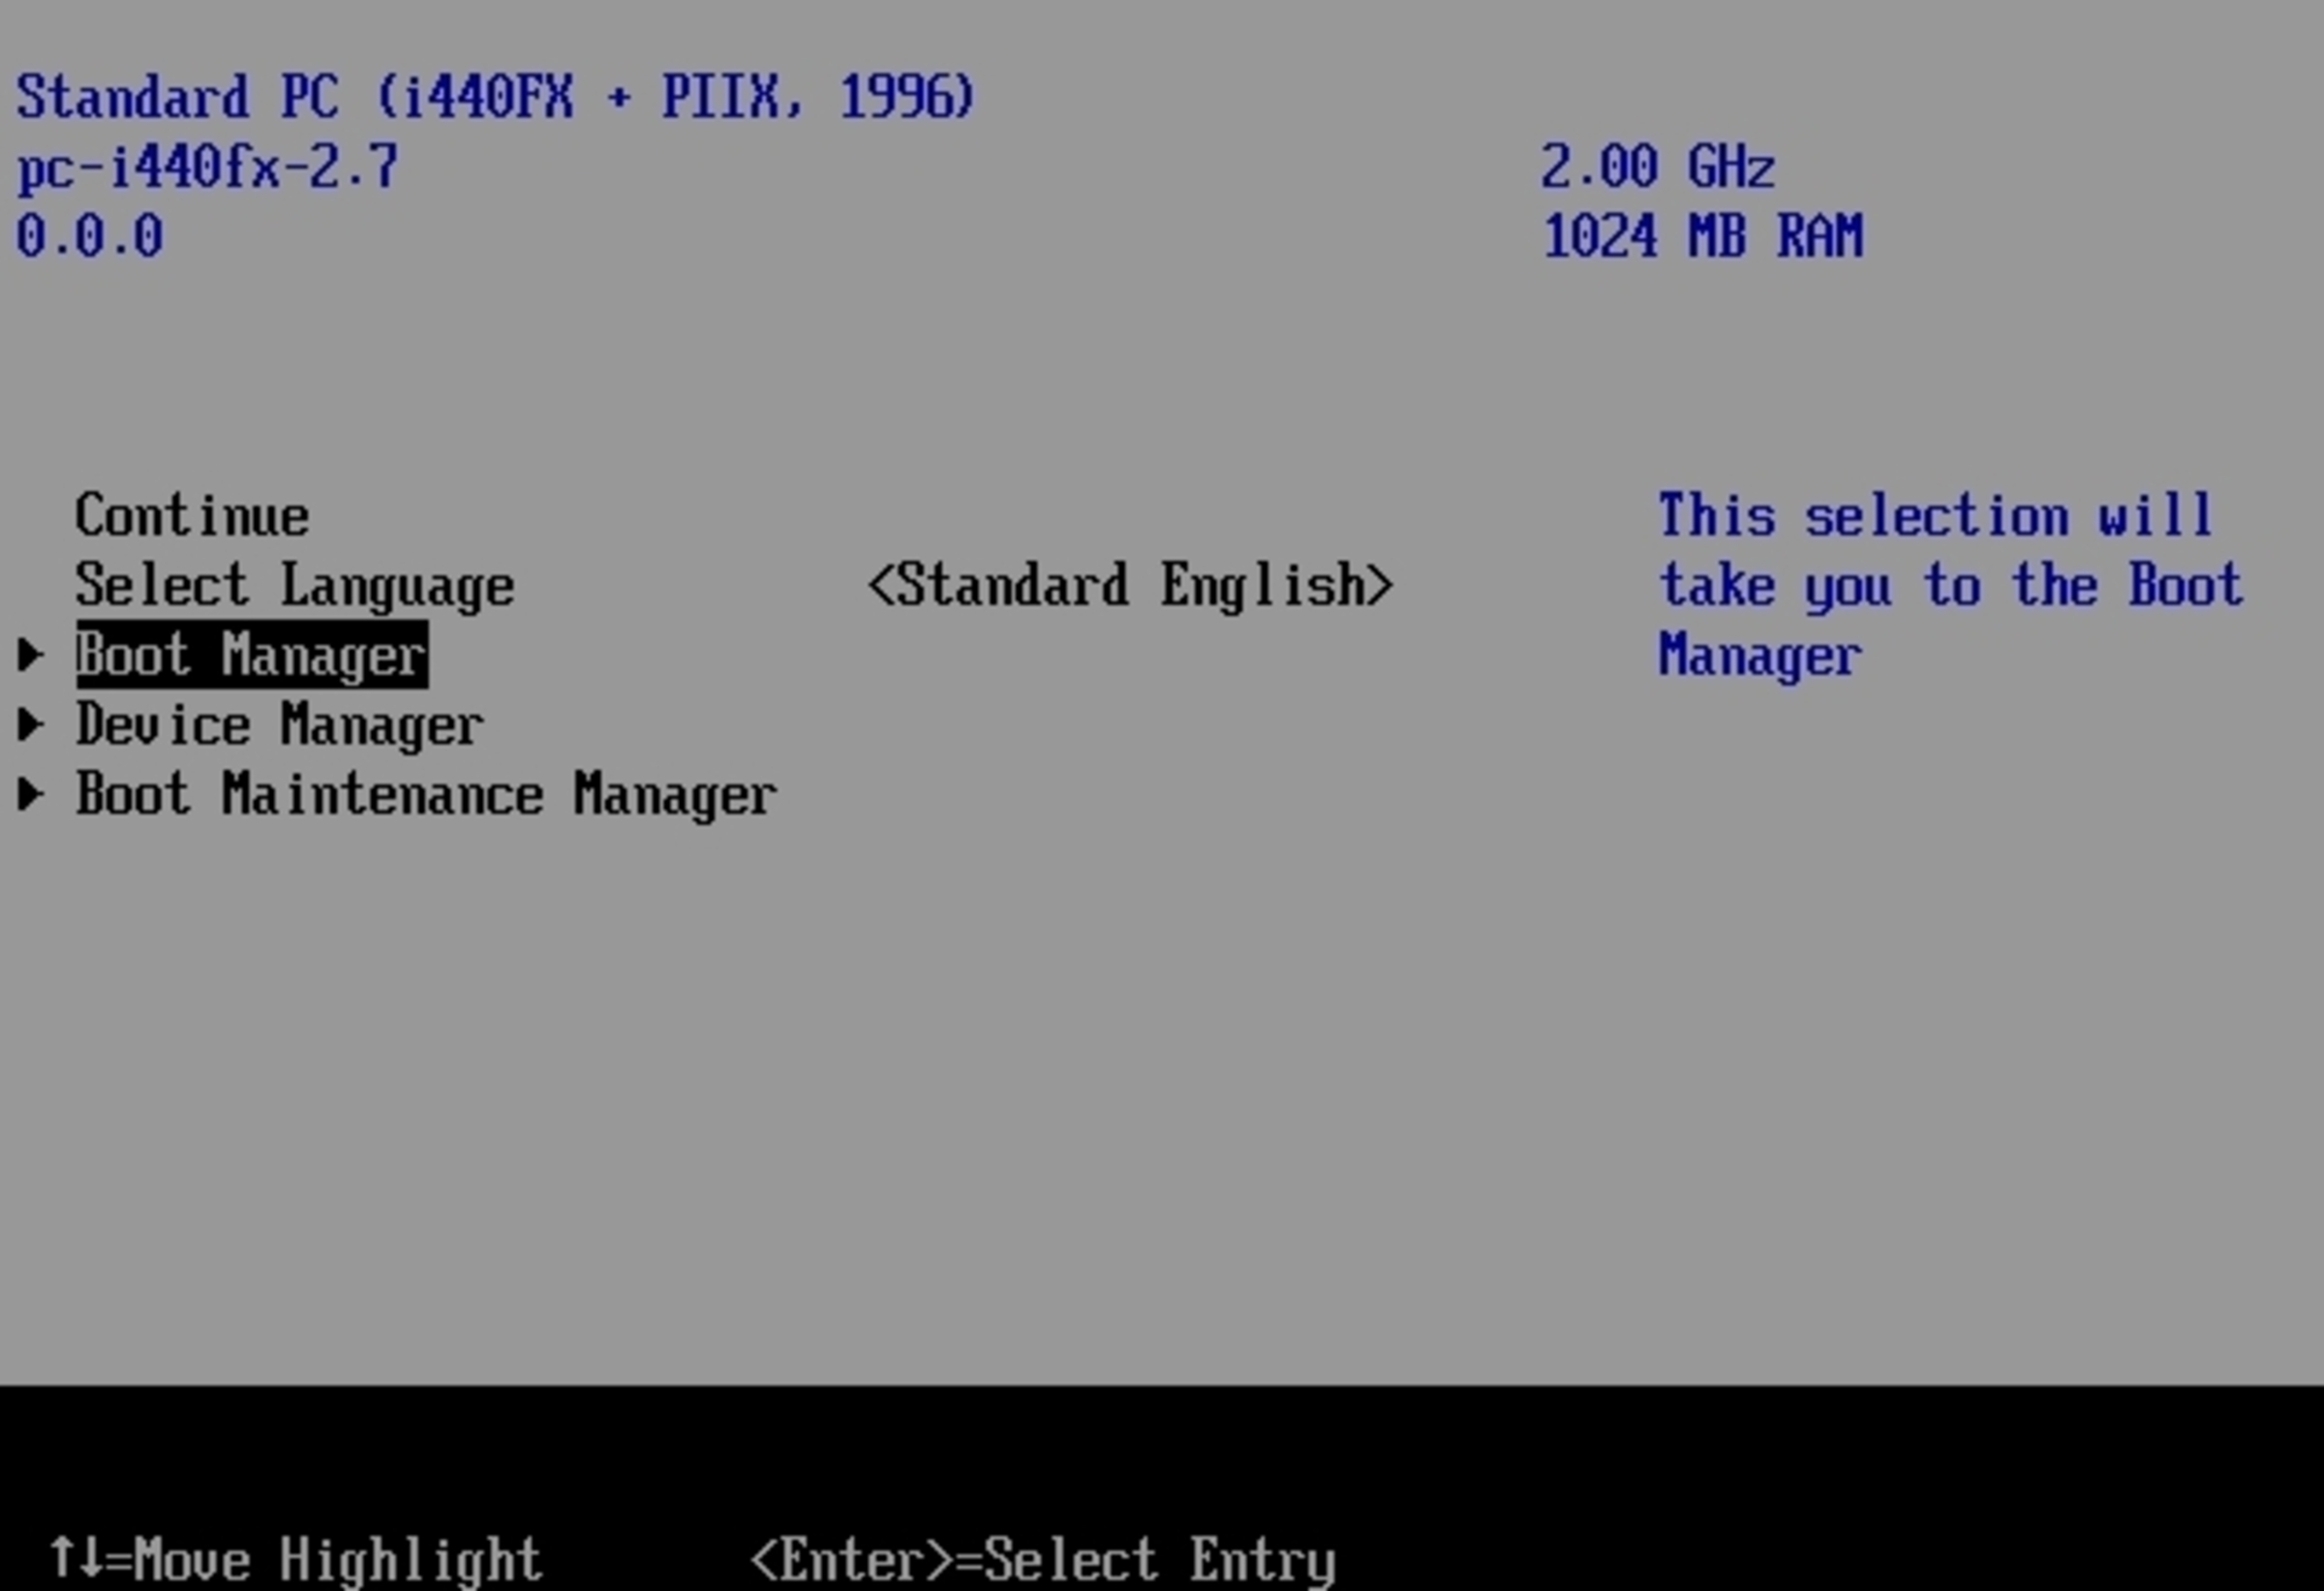
\includegraphics[resolution=600]{ovmf-setup}
	\caption{Pannello di configurazione di un firmware UEFI (OVMF)}
	\label{fig:ovmf-setup}
\end{figure}

Se si tratta di un firmware \texttt{UEFI} dobbiamo adesso vedere se è possibile disattivare il Secure Boot. Non esiste un modo standard per disattivare il Secure Boot, quindi non si può dare una procedura precisa per farlo. Inoltre, non è nemmeno certo che sia possibile (su alcuni computer, è impossibile disabilitare il Secure Boot). Su altri ancora è possibile che, nonostante sia presente un firmware \texttt{UEFI}, il Secure Boot non sia stato implementato e quindi non c'è alcun bisogno di disattivarlo. In altri sistemi ancora, è possibile che non esista alcuna voce per disattivare il Secure Boot ma che ne esista una per passare dalla modalità \texttt{UEFI} alla modalità \texttt{BIOS} legacy. Passando alla modalità \texttt{BIOS} ovviamente si disattiva anche il Secure Boot. Ancora: per accordi che ci sono stati tra Microsoft, Linux Foundation e i produttori di hardware, in alcuni sistemi è possibile che non ci sia la necessità di disattivare il Secure Boot in quanto le firme digitali per avviare un sistema Linux sono già state inserite all'interno del database del firmware. Infine, in alcuni (pochi) sistemi, per vecchi accordi tra Microsoft e i produttori di hardware, potrebbe essere totalmente impossibile avviare un qualsiasi sistema operativo che non sia Windows. In quest'ultimo caso, seppur raro, c'è poco da fare: Debian non può essere installato --- potete però usare una macchina virtuale dentro Windows!

Se si è modificata qualche impostazione dal pannello del firmware, bisogna ricordarsi di salvare prima di uscire!
